\chapter{Štatistické grafy a vyhodnotenie bitových tokov}

Táto kapitola sa primárne venuje testovaniu bitového toku generovaného kvantovým generátorom náhodných čísel (\textit{QRNG}), ktorý predstavuje hlavnú skúmanú súčasť tejto práce.
Cieľom analýzy je overiť, či výstup QRNG vykazuje vlastnosti očakávané od kvalitného zdroja náhodnosti, teda či sa generované bity správajú ako náhodné dáta bez detekovateľnej štruktúry, systematického skreslenia alebo predikovateľnosti.

Na účely objektívneho vyhodnotenia je bitový tok generovaný kvantovým generátorom náhodných čísel porovnávaný s nasledujúcimi referenčnými zdrojmi:
\begin{itemize}
  \item \textbf{Bitový tok generovaný pseudonáhodným generátorom jazyka Python} bol zvolený ako kvalitná porovnávacia referencia.
  Generátor používaný v štandardnej knižnici jazyka Python je založený na algoritme \textit{Mersenne Twister}, ktorý patrí medzi najpoužívanejšie pseudonáhodné generátory v softvérových aplikáciách.
  Ide o deterministický algoritmus založený na rekurentnej transformácii vnútorného stavu generátora pomocou lineárnych operácií nad binárnymi vektormi.
  Algoritmus je navrhnutý tak, aby mal veľmi dlhú periódu ($2^{19937}-1$) a dobré štatistické vlastnosti, ktoré umožňujú jeho použitie v širokom spektre simulácií a numerických výpočtov.
  Hoci nejde o fyzikálne náhodný zdroj, generovaný bitový tok sa v mnohých štatistických testoch správa podobne ako skutočne náhodná sekvencia, čo z neho robí vhodnú referenciu pre porovnanie s kvantovým generátorom náhodných čísel.

  Podrobný opis princípu fungovania algoritmu Mersenne Twister je uvedený napríklad v dokumentácii jazyka Python\cite{python_random_docs} a v pôvodnej publikácii autorov algoritmu\cite{matsumoto1998mersenne}.

  \item \textbf{Bitový tok generovaný zámerne slabým lineárnym kongruenčným generátorom} je v tejto práci použitý ako kontrolná vzorka, ktorej úlohou je overiť schopnosť použitých testov odhaliť nenáhodné a deterministické správanie.
  Lineárny kongruenčný generátor patrí medzi najjednoduchšie pseudonáhodné generátory a je definovaný rekurentným vzťahom

  \[
    x_{n+1} = (a x_n + c) \bmod m,
  \]

  kde $x_n$ predstavuje aktuálny stav generátora, $a$ je multiplikatívny koeficient, $c$ je inkrement a $m$ je modul určujúci rozsah hodnôt.
  Každá ďalšia hodnota sekvencie je teda deterministicky odvodená z predchádzajúcej hodnoty pomocou lineárnej transformácie a operácie modulo.
  Hoci takýto prístup umožňuje veľmi rýchlu implementáciu generátora, je známe, že lineárne kongruenčné generátory vykazujú rôzne štatistické nedostatky a korelácie medzi generovanými hodnotami \cite{knuth1997art}.
  \end{itemize}

Takto zvolený prístup umožňuje posudzovať vlastnosti QRNG nielen izolovane, ale aj v kontexte kvalitného pseudonáhodného generátora a zároveň voči kontrolnej vzorke, pri ktorej sa očakáva zlyhanie vo viacerých testoch náhodnosti.

Jednotlivé časti tejto kapitoly prezentujú rovnaký typ testu pre všetky tri zdroje v rovnakom poradí, aby bolo možné ich vlastnosti priamo porovnať.








\section{Analýza rozdelenia bitového toku}

V tejto časti je analyzovaná stabilita bitového toku v čase pomocou jeho rozdelenia na viacero častí.
Analyzovaný bitový tok je rozdelený na desať rovnakých segmentov a každý segment je vyhodnotený samostatne.
Cieľom testu je overiť, či sa štatistické vlastnosti generovaného bitového toku nemenia v priebehu generovania a či generátor nevykazuje lokálne skreslenie.

Pre každý segment sú sledované najmä tieto charakteristiky:
podiel núl ($p_{\text{nuly}}$), podiel jednotiek ($p_{\text{jednotky}}$) a odchýlka od ideálneho pomeru $0{,}5$.
Grafické znázornenie výsledkov umožňuje vizuálne posúdiť stabilitu generátora.
Stĺpcový graf zobrazuje hodnoty $p_{\text{nuly}}$ a $p_{\text{jednotky}}$ pre jednotlivé segmenty bitového toku, zatiaľ čo čiarový graf znázorňuje hodnotu odchýlky.

Na obr.~\ref{fig:2Biasqrng} je zobrazená analýza rozdelenia bitového toku generovaného kvantovým generátorom náhodných čísel.
Z grafu je možné pozorovať, že podiel núl aj jednotiek v jednotlivých segmentoch zostáva veľmi blízky ideálnemu pomeru $0{,}5$.
Hodnota odchýlky je nízka a nevykazuje výrazné výkyvy medzi jednotlivými segmentmi.
Takéto správanie naznačuje stabilné generovanie bitov bez výrazných lokálnych skreslení.

\begin{figure}[H]
  \centering
  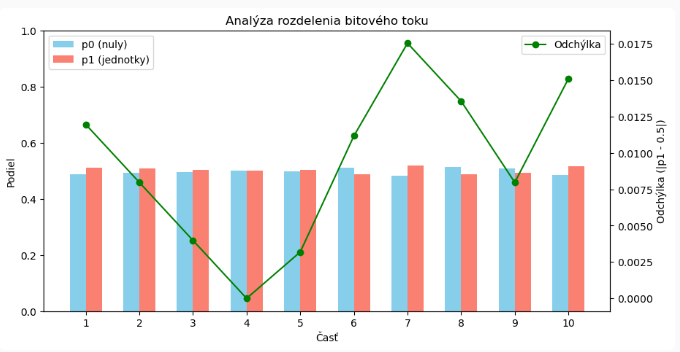
\includegraphics[width=0.85\textwidth]{images/2Biasqrng}
  \caption{Analýza rozdelenia bitového toku QRNG}
  \label{fig:2Biasqrng}
\end{figure}

Na obr.~\ref{fig:2Biasprng} je zobrazená rovnaká analýza pre bitový tok generovaný pseudonáhodným generátorom jazyka Python.
Graf ukazuje podobný charakter rozdelenia bitov ako v prípade kvantového generátora.
Podiel núl a jednotiek sa síce medzi jednotlivými segmentmi mierne mení, avšak hodnoty zostávajú v blízkosti ideálneho pomeru.
V niektorých segmentoch možno pozorovať mierne vyššiu odchýlku, čo je pri pseudonáhodných generátoroch a konečných vzorkách očakávané.

\begin{figure}[H]
  \centering
  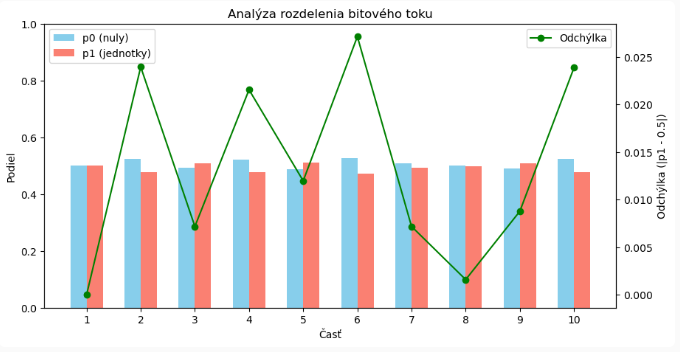
\includegraphics[width=0.85\textwidth]{images/2Biasprng}
  \caption{Analýza rozdelenia bitového toku generovaného pseudonáhodným generátorom jazyka Python}
  \label{fig:2Biasprng}
\end{figure}

Na obr.~\ref{fig:2Biaslcg} je zobrazená analýza pre bitový tok generovaný kontrolným lineárnym kongruenčným generátorom.
Na rozdiel od predchádzajúcich generátorov graf vykazuje takmer dokonale konštantné hodnoty podielu núl aj jednotiek vo všetkých segmentoch.
Odchýlka je prakticky nulová v celej analyzovanej sekvencii.
Takáto pravidelnosť je však pri skutočne náhodných sekvenciách nepravdepodobná a naznačuje deterministickú štruktúru generovaného bitového toku.

\begin{figure}[H]
  \centering
  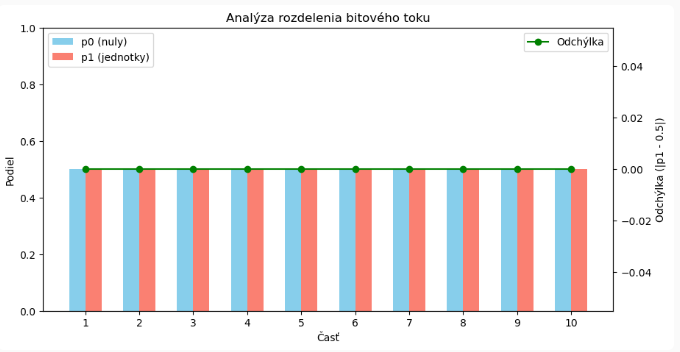
\includegraphics[width=0.85\textwidth]{images/2Biaslcg}
  \caption{Analýza rozdelenia bitového toku generovaného kontrolným lineárnym kongruenčným generátorom}
  \label{fig:2Biaslcg}
\end{figure}

Porovnanie grafov ukazuje výrazný rozdiel medzi jednotlivými generátormi.
Bitový tok generovaný kvantovým generátorom náhodných čísel vykazuje stabilné správanie s malými fluktuáciami medzi jednotlivými segmentmi.
Pseudonáhodný generátor jazyka Python vykazuje podobný charakter rozdelenia, avšak s mierne väčšími odchýlkami.
Naopak kontrolný lineárny kongruenčný generátor produkuje takmer dokonale rovnomerné rozdelenie bitov v každom segmente, čo poukazuje na deterministický charakter generátora.







\section{Analýza rozdelenia bitového toku po extrakcii entropie pomocou MD5}

V tejto časti je analyzovaný vplyv extrakcie entropie na vlastnosti generovaného bitového toku.
Na transformáciu pôvodného bitového toku bola použitá kryptografická hašovacia funkcia MD5, ktorá slúži ako jednoduchý mechanizmus na tzv. whitening alebo extrakciu entropie.

Princíp tejto transformácie spočíva v tom, že vstupné bloky bitov sú spracované hašovacou funkciou, ktorá vytvára nový výstupný bitový tok.
Takáto transformácia dokáže rozptýliť lokálne štruktúry a zvyškové korelácie v dátach.
Dôležitou vlastnosťou však je, že extrakcia entropie nedokáže vytvoriť náhodnosť sama o sebe.

Na obr.~\ref{fig:3md5qrng} je zobrazená analýza rozdelenia bitového toku generovaného kvantovým generátorom náhodných čísel po aplikovaní MD5 transformácie.
Z grafu je možné pozorovať, že podiel núl aj jednotiek v jednotlivých segmentoch zostáva veľmi blízky ideálnemu pomeru.
Hodnota odchýlky je nízka a stabilná naprieč celou sekvenciou, čo naznačuje dobré štatistické vlastnosti výsledného bitového toku.

\begin{figure}[H]
  \centering
  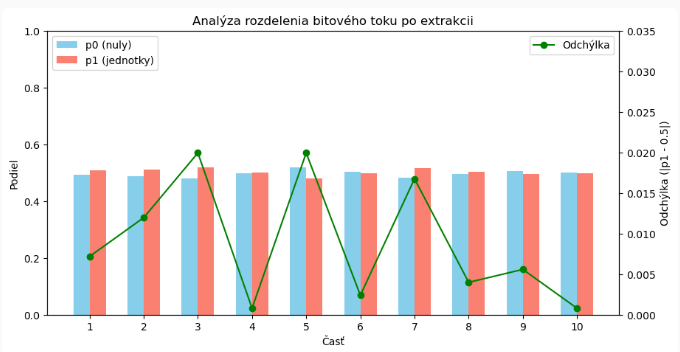
\includegraphics[width=0.85\textwidth]{images/3md5qrng}
  \caption{Analýza rozdelenia bitového toku generovaného kvantovým generátorom náhodných čísel po extrakcii entropie pomocou MD5}
  \label{fig:3md5qrng}
\end{figure}

Na obr.~\ref{fig:3md5prng} je zobrazená rovnaká analýza pre bitový tok generovaný pseudonáhodným generátorom jazyka Python.
Graf ukazuje, že transformácia pomocou MD5 nemení zásadne charakter rozdelenia bitov.
Podiel núl a jednotiek zostáva v jednotlivých segmentoch približne vyvážený a hodnoty odchýlky sú podobné ako v prípade pôvodného bitového toku.

\begin{figure}[H]
  \centering
  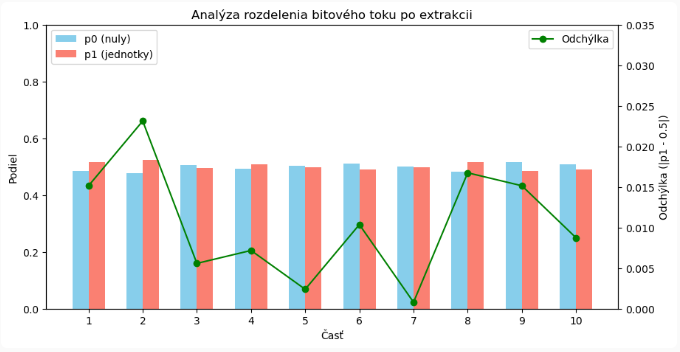
\includegraphics[width=0.85\textwidth]{images/3md5prng}
  \caption{Analýza rozdelenia bitového toku generovaného pseudonáhodným generátorom jazyka Python po extrakcii entropie pomocou MD5}
  \label{fig:3md5prng}
\end{figure}

Na obr.~\ref{fig:3md5lcg} je zobrazená analýza pre bitový tok generovaný kontrolným lineárnym kongruenčným generátorom.
Aj po aplikovaní MD5 transformácie zostáva rozdelenie bitov výrazne systematické a odchýlka vykazuje konzistentné hodnoty.
Tento výsledok naznačuje, že extrakcia entropie nedokáže odstrániť deterministický charakter generátora.

\begin{figure}[H]
  \centering
  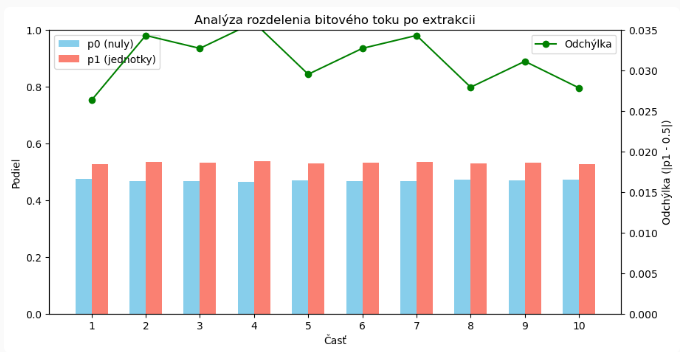
\includegraphics[width=0.85\textwidth]{images/3md5lcg}
  \caption{Analýza rozdelenia bitového toku generovaného kontrolným lineárnym kongruenčným generátorom po extrakcii entropie pomocou MD5}
  \label{fig:3md5lcg}
\end{figure}

Porovnanie výsledkov ukazuje, že extrakcia entropie pomocou hašovacej funkcie MD5 je účinná najmä v prípade zdrojov, ktoré už obsahujú určitú mieru náhodnosti.
Pri kvantovom generátore transformácia pomáha rozptýliť drobné lokálne nerovnováhy a zlepšuje kvalitu výsledného bitového toku.

Pseudonáhodný generátor jazyka Python vykazuje po transformácii podobné vlastnosti ako pred transformáciou, keďže jeho výstup už má dobré štatistické vlastnosti.

Naopak pri kontrolnom lineárnom kongruenčnom generátore sa potvrdzuje, že samotná hašovacia transformácia nedokáže odstrániť deterministický charakter zdroja.

\textit{Extrakcia entropie založená na hašovaní nemôže zvýšiť entropiu nad úroveň entropie, ktorá je už prítomná vo vstupnom zdroji.}









\section{NIST testy}


V tejto časti boli použité základné štatistické testy inšpirované metodikou NIST.
Tieto testy overujú rôzne vlastnosti bitového toku a pomáhajú odhaliť systematické odchýlky alebo jednoduchú nenáhodnú štruktúru.

Použité boli nasledujúce testy:

\begin{itemize}
  \item \textbf{Test vyváženosti bitov (TVB)} -- overuje, či je počet núl a jednotiek približne vyvážený,

  \item \textbf{Test behov bitov (TBB)} -- overuje, či prechody medzi hodnotami 0 a 1 nastávajú primeranou frekvenciou; príliš veľa alebo príliš málo behov môže signalizovať prítomnosť štruktúry,

  \item \textbf{Test kumulatívneho súčtu (TKS)} -- sleduje, či kumulatívny súčet bitov nevykazuje výrazný drift od nuly, čo môže naznačovať pretrvávajúcu nerovnováhu v sekvencii.
\end{itemize}



\begin{table}[H]
  \centering
  \caption{NIST pre QRNG}
  \label{tab:nist_qrng}
  \begin{tabular}{lccc}
    \toprule
    \textbf{Test} & \textbf{Hranica} & \textbf{p-hodnota} & \textbf{Stav} \\
    \midrule
    Test vyváženosti bitov (TVB)   & $p > 0{,}1$ & 0,54376 & Vyhovel \\
    Test behov bitov (TBB)         & $p > 0{,}1$ & 0,99814 & Vyhovel \\
    Test kumulatívneho súčtu (TKS) & $p > 0{,}1$ & 0,38645 & Vyhovel \\
    \bottomrule
  \end{tabular}

\end{table}

\begin{table}[H]
  \centering
  \caption{NIST generátor jazyka Python}
  \label{tab:nist_prng}
  \begin{tabular}{lccc}
    \toprule
    \textbf{Test} & \textbf{Hranica} & \textbf{p-hodnota} & \textbf{Stav} \\
    \midrule
    Test vyváženosti bitov (TVB)   & $p > 0{,}1$ & 0,08325 & Nevyhovel \\
    Test behov bitov (TBB)         & $p > 0{,}1$ & 0,49923 & Vyhovel \\
    Test kumulatívneho súčtu (TKS) & $p > 0{,}1$ & 0,07859 & Nevyhovel \\
    \bottomrule
  \end{tabular}

\end{table}

\begin{table}[H]
  \centering
  \caption{NIST pre kontrolnú vzorku}
  \label{tab:nist_lcg}
  \begin{tabular}{lccc}
    \toprule
    \textbf{Test} & \textbf{Hranica} & \textbf{p-hodnota} & \textbf{Stav} \\
    \midrule
    Test vyváženosti bitov (TVB)   & $p > 0{,}1$ & 1,00000 & Vyhovel \\
    Test behov bitov (TBB)         & $p > 0{,}1$ & 0,00000 & Nevyhovel \\
    Test kumulatívneho súčtu (TKS) & $p > 0{,}1$ & 0,99288 & Vyhovel \\
    \bottomrule
  \end{tabular}

\end{table}

Bitový tok generovaný kvantovým generátorom náhodných čísel úspešne vyhovel všetkým implementovaným štatistickým testom.
Získané p-hodnoty pre test vyváženosti bitov, test behov bitov aj test kumulatívneho súčtu presahujú stanovenú hranicu $p>0{,}1$.
Tieto výsledky neindikujú štatisticky významnú nerovnováhu medzi nulami a jednotkami, anomálnu štruktúru behov ani výrazný drift kumulatívneho súčtu.
Možno teda konštatovať, že analyzovaný bitový tok nevykazuje na testovanej vzorke zjavné štatistické nepravidelnosti.

Bitový tok generovaný pseudonáhodným generátorom jazyka Python poskytol zmiešané výsledky.
Kým test behov bitov vyhovel stanovenej podmienke, test vyváženosti bitov a test kumulatívneho súčtu nedosiahli požadovanú hranicu úspešnosti.
Takéto výsledky naznačujú, že hoci sa tento generátor vo všeobecnosti správa podobne ako náhodný zdroj, pri konečných vzorkách sa môžu objaviť menšie štatistické odchýlky.

Bitový tok generovaný kontrolným lineárnym kongruenčným generátorom vykázal charakteristický vzor správania.
Hoci vyhovel testu vyváženosti bitov aj testu kumulatívneho súčtu, nevyhovel testu behov bitov.
Tento výsledok ilustruje dôležitý princíp testovania náhodnosti: úspech v niekoľkých štatistických testoch ešte neznamená skutočnú náhodnosť.
V danom prípade bol síce počet núl a jednotiek vyvážený, avšak ich usporiadanie vykazovalo silnú deterministickú štruktúru, ktorú test behov bitov dokázal odhaliť.










\section{Next-bit test}


Next-bit test skúma, či je možné pomocou modelu strojového učenia predpovedať nasledujúci bit na základe predchádzajúcich bitov.
Ak model dosahuje výrazne lepšie výsledky než náhodné hádanie, analyzovaná sekvencia môže obsahovať lokálnu štruktúru, ktorú je možné naučiť.

Vyhodnocované v tabuľke\ref{tab:nextbit_summary} boli tieto metriky:
\begin{itemize}
  \item \textbf{Presnosť predikcie (PP)} -- podiel správne predikovaných nasledujúcich bitov; hodnota blízka 0,5 zodpovedá náhodnému správaniu,

  \item \textbf{Vyvážená presnosť (VP)} -- presnosť korigovaná vzhľadom na prípadnú nevyváženosť medzi triedami 0 a 1,

  \item \textbf{Schopnosť rozlišovania tried (SRT)} -- miera schopnosti modelu oddeľovať dve triedy; hodnota okolo 0,5 znamená absenciu prediktívnej sily,

  \item \textbf{Logaritmická strata predikcie (LSP)} -- miera kvality pravdepodobnostnej predikcie; pri nepredikovateľnom binárnom prúde býva blízka hodnote 0,693,

  \item \textbf{Štatistická významnosť výsledku (SV)} -- určuje, či je výkon modelu štatisticky významne lepší než náhodné hádanie.
\end{itemize}

Kvalitný náhodný bitový tok by mal viesť k výsledkom blízkym úrovni náhody.
Naopak slabý pseudonáhodný zdroj môže vykazovať zvýšenú predikovateľnosť.


\begin{table}[H]
  \centering
  \caption{Výsledky testu predikcie nasledujúceho bitu a interpretácia použitých metrík}
  \label{tab:nextbit_summary}
  \begin{tabular}{lccccccccc}
    \toprule
    \textbf{Zdroj}  & \textbf{PP} & \textbf{VP} & \textbf{SRT} & \textbf{LSP} & \textbf{SV} \\
    \midrule
    QRNG            & 0,49137 & 0,49142 & 0,48362 & 0,69388 & 0,91584 \\
    Python PRNG     & 0,49728 & 0,49301 & 0,49722 & 0,69340 & 0,67089 \\
    Kontrolný LCG   & 1,00000 & 1,00000 & 1,00000 & 0,00021 & 0,00000 \\
    \midrule
    \textbf{Minimum}            & 0 & 0 & 0 & 0 & 0 \\
    \textbf{Maximum}            & 1 & 1 & 1 & $\infty$ & 1 \\
    \textbf{Predpokladáme} & $\approx0,5$ & $\approx0,5$ & $\approx0,5$ & $\approx0,693$ & $>0,05$ \\
    \bottomrule
  \end{tabular}
\end{table}

Výsledky testu predikcie nasledujúceho bitu sú doplnené aj grafickým znázornením.
Na obr.~\ref{fig:1Nextqrng} je zobrazený graf pre bitový tok generovaný kvantovým generátorom náhodných čísel.
Graf pre bitový tok generovaný pseudonáhodným generátorom jazyka Python je uvedený na obr.~\ref{fig:1Nextprng}.
Posledný graf, zobrazený na obr.~\ref{fig:1Nextlcg}, prezentuje výsledky kontrolnej vzorky.
Na vyhodnotenie modelu bola použitá metóda \textit{10-fold cross-validation}, pri ktorej je dataset rozdelený na desať rovnakých častí.

Každý graf obsahuje stĺpcový diagram, v ktorom sú pre jednotlivé foldy zobrazené dve hodnoty:
\textit{Model Accuracy}, teda presnosť predikčného modelu, a \textit{Majority Baseline}, ktorá predstavuje jednoduchý referenčný prístup spočívajúci v predikcii najčastejšej triedy.
Tento baseline slúži ako porovnávacia referencia, ktorá umožňuje overiť, či model skutočne dokáže extrahovať informáciu z analyzovaného bitového toku.

\begin{figure}[htbp]
  \centering
  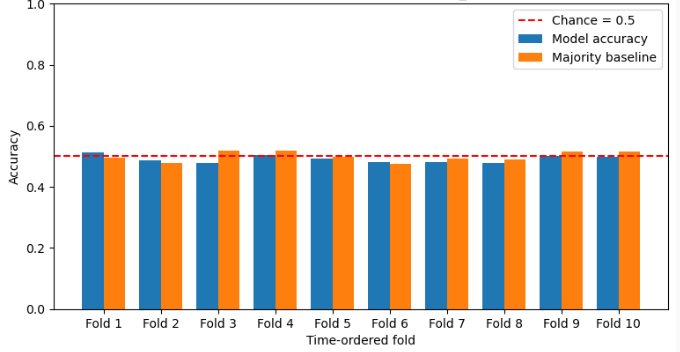
\includegraphics[width=0.85\textwidth]{images/1Nenxtqrng}
  \caption{bitový tok generovaný kvantovým generátorom náhodných čísel (QRNG)}
  \label{fig:1Nextqrng}
\end{figure}

\begin{figure}[htbp]
  \centering
  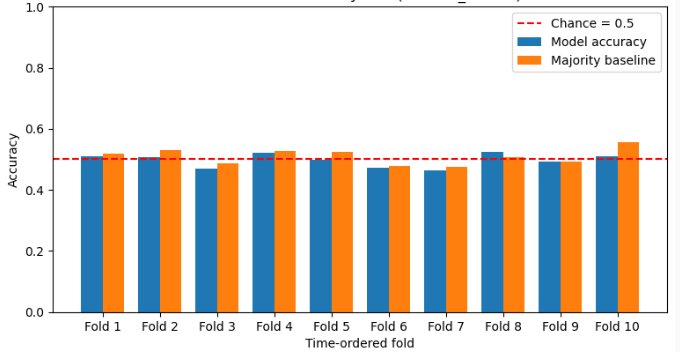
\includegraphics[width=0.85\textwidth]{images/1Nextprng}
  \caption{bitový tok generovaný pseudonáhodným generátorom jazyka Python.}
  \label{fig:1Nextprng}
\end{figure}

\begin{figure}[htbp]
  \centering
  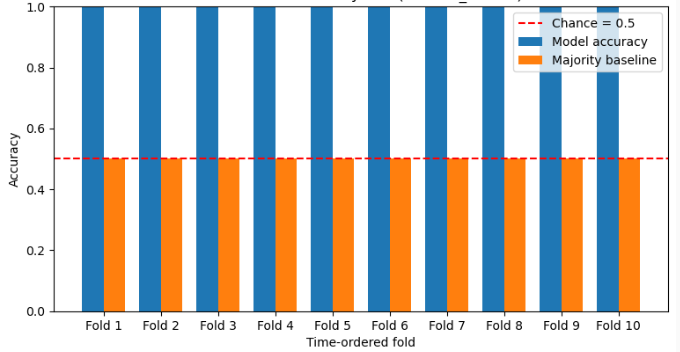
\includegraphics[width=0.85\textwidth]{images/1Nextlcg}
  \caption{kontrolná vzorka}
  \label{fig:1Nextlcg}
\end{figure}


Výsledky ukazujú, že pri bitových tokoch generovaných kvantovým generátorom náhodných čísel a pseudonáhodným generátorom jazyka Python model nedosahuje výkon lepší než náhodné hádanie.
V oboch prípadoch sa hodnoty presnosti predikcie (PP), vyváženej presnosti (VP) aj schopnosti rozlišovania tried (SRT) nachádzajú veľmi blízko hodnoty 0,5.
Zároveň vysoké hodnoty štatistickej významnosti výsledku (SV) neindikujú štatisticky významnú predikčnú schopnosť modelu.
Takéto výsledky naznačujú, že analyzované bitové toky neobsahujú ľahko naučiteľnú lokálnu štruktúru, ktorú by bolo možné využiť na spoľahlivú predikciu nasledujúceho bitu.

Naopak, pri kontrolnom lineárnom kongruenčnom generátore model dosiahol perfektnú predikciu.
Hodnoty presnosti predikcie (PP), vyváženej presnosti (VP) aj schopnosti rozlišovania tried (SRT) dosiahli maximálnu hodnotu 1,0.
Zároveň bola zaznamenaná veľmi nízka hodnota logaritmickej straty predikcie (LSP) spolu s nulovou hodnotou štatistickej významnosti výsledku (SV).
Takéto výsledky jednoznačne indikujú prítomnosť silnej deterministickej štruktúry v analyzovanom bitovom toku, ktorú je model schopný spoľahlivo identifikovať a využiť pri predikcii nasledujúceho bitu.



\section{Markovov test}


Markovov test odhaduje, či nasledujúci bit závisí od bezprostredne predchádzajúceho vzoru bitov.
Ide o jednoduchší test lokálnej závislosti narozdiel od Next-bit testu založený na strojovom učení, no je užitočný pri detekcii opakujúcich sa krátkodosahových vzorov.

Vyhodnocované v tabulke\ref{tab:markov} boli tieto metriky:

\begin{itemize}
  \item \textbf{presnosť predikcie (PP)} -- vyjadruje podiel správne predikovaných nasledujúcich bitov. Hodnota blízka 0,5 naznačuje správanie zodpovedajúce náhodnému hádaniu.

  \item \textbf{vyvážená presnosť (VP)} -- predstavuje presnosť predikcie korigovanú vzhľadom na prípadnú nevyváženosť medzi triedami bitov 0 a 1. Tento ukazovateľ poskytuje spoľahlivejšie hodnotenie výkonu modelu pri nevyvážených dátach.

  \item \textbf{p-hodnota (SV)} -- určuje, či je pozorovaná úspešnosť predikcie štatisticky významne lepšia než náhodné hádanie. Vysoká hodnota naznačuje, že model nevyužíva žiadnu detegovateľnú štruktúru v bitovom toku.

  \item \textbf{počet testovaných predikcií (PTP)} -- udáva celkový počet vyhodnotených predikcií použitých pri výpočte metrík. Väčší počet predikcií zvyšuje spoľahlivosť a stabilitu získaných výsledkov.
\end{itemize}


\begin{table}[H]
  \centering
  \caption{Výsledky Markovovho testu}
  \label{tab:markov}
  \begin{tabular}{lcccc}
    \toprule
    \textbf{Zdroj} & \textbf{PP} & \textbf{VP} & \textbf{SV} & \textbf{PTP} \\
    \midrule
    QRNG           & 0,48764 & 0,48772 & 0,93733 & 3761 \\
    Python PRNG    & 0,49003 & 0,48972 & 0,89238 & 3761 \\
    Kontrolný LCG  & 1,00000 & 1,00000 & 0,00000 & 3761 \\
    \midrule
    Predpoklad & $\approx 0,5$ & $\approx 0,5$ & $> 0,1$ & závisí od vzorky \\
    \bottomrule
  \end{tabular}
\end{table}

Pri bitovom toku generovanom kvantovým generátorom náhodných čísel bola dosiahnutá hodnota presnosti predikcie (PP) 0,48764 pri vysokej hodnote p-hodnoty (SV) 0,93733, čo znamená, že prediktor nebol úspešnejší než náhodné hádanie.
Tento výsledok naznačuje, že výstup QRNG neobsahuje detegovateľné krátkodosahové závislosti medzi susediacimi bitmi.

Bitový tok generovaný pseudonáhodným generátorom jazyka Python dosiahol podobné výsledky.
Presnosť predikcie (PP) bola 0,49003 a p-hodnota (SV) dosiahla hodnotu 0,89238.
Ani v tomto prípade sa nepreukázala využiteľná prediktívna štruktúra.

Naopak pri bitovom toku generovanom kontrolným lineárnym kongruenčným generátorom bola dosiahnutá perfektná predikovateľnosť.
Presnosť predikcie aj vyvážená presnosť dosiahli hodnotu 1,0 a p-hodnota bola nulová.
Tento výsledok jednoznačne potvrdzuje prítomnosť silnej deterministickej štruktúry v analyzovanom bitovom toku.



\section{Zhrnutie výsledkov}

%Hlavným cieľom tejto práce bolo ukázať, že kvantový generátor náhodných čísel nepredstavuje iba teoretický koncept, ale že jeho vlastnosti je možné overiť aj prostredníctvom merateľných štatistických dôkazov.
%Cieľom preto nebolo len implementovať generátor, ale predovšetkým systematicky analyzovať kvalitu generovaného bitového toku pomocou viacerých nezávislých testovacích metód.

Na overenie kvality generovaných bitových tokov bol kvantový generátor porovnávaný s dvoma referenčnými zdrojmi.
Prvým bol pseudonáhodný generátor jazyka Python, ktorý je v praxi považovaný za veľmi kvalitný algoritmický generátor a vo väčšine štatistických testov vykazuje veľmi dobré výsledky.
Druhým zdrojom bol kontrolný lineárny kongruenčný generátor, ktorý bol použitý ako referenčná vzorka s očakávaným deterministickým správaním.

Na základe vykonaných testov sa potvrdilo očakávanie, že bitový tok generovaný kvantovým generátorom bude vykazovať vlastnosti typické pre náhodné sekvencie a zároveň dosahovať lepšie alebo minimálne porovnateľné výsledky ako referenčné vzorky.
Výsledky štatistických testov aj prediktívnych modelov ukázali, že z kvantového systému je možné extrahovať entropiu, ktorá sa následne dá použiť na generovanie náhodných čísel.
Bitový tok generovaný kvantovým generátorom nevykazoval detekovateľnú predikovateľnú štruktúru a v testoch sa správal v súlade s očakávaným správaním náhodného zdroja.

Dôležitým zistením práce je aj to, že na spoľahlivé hodnotenie kvality náhodnosti je potrebné použiť viacero rôznych testovacích metód.
V niektorých jednoduchších štatistických ukazovateľoch sa napríklad kontrolný lineárny kongruenčný generátor javil ako dokonale vyvážený zdroj bitov.
Takáto dokonalá rovnováha medzi nulami a jednotkami však v skutočnosti nie je znakom vysokej entropie.
Práve naopak, skutočne náhodné sekvencie prirodzene obsahujú malé fluktuácie a lokálne odchýlky.
Až kombinácia štatistických testov, prediktívnych modelov a analýzy štruktúry bitového toku umožňuje spoľahlivo identifikovať deterministické vzory.

Ďalším dôležitým poznatkom práce je úloha extrakcie entropie.
Transformácie založené na kryptografických hašovacích funkciách dokážu rozptýliť lokálne štruktúry a odstrániť niektoré systematické odchýlky, avšak nedokážu umelo vytvoriť novú entropiu.
Extrakcia entropie dokáže iba využiť a rozložiť entropiu, ktorá je už prítomná vo vstupnom fyzikálnom procese.
Preto je pri návrhu generátorov náhodných čísel kľúčové identifikovať spoľahlivý fyzikálny zdroj entropie.


